\section{Background}
%\subsection{Stages of Self-Tracking}
In recent years, Personal Informatics or Quantified Self (QS) tools have received an increasing interest in the field of human-computer interaction with the introduction of low-cost mobile applications, wearables and advances in sensor technologies. Personal Informatics help people understand themselves through self-tracking of “personally relevant information for the purpose of self-reflection and gaining self-knowledge” \cite{Li2010}. 

Researchers have proposed different models for understanding, how self-trackers concretely use Personal Informatics tools over time. Li et al. proposed the cascading five-staged \textit{Personal Informatics Model} describing, how self-trackers transition between: (1) \textit{Preparation} (determining variables, tools and frequency of tracking), (2) \textit{collection} (logging data), (3) \textit{integration} (preparing data for reflection e.g. by aggregating and analysing data), (4) \textit{reflection} (examining data to gain self-knowledge) and (5) \textit{action} (deciding what to do with said knowledge) \cite{Li2010}. 

Little is known about self-tracking practices around telehealth systems in the health context, but we found that despite telehealth does not completely reflect the practices of Personal Informatics (because there are multiple stakeholders/users in telehealth), the above-mentioned stages still apply. We have illustrated the differences between stakeholders’ roles in Personal Informatics and Telehealth on Figure \ref{fig:StakeholdersModel}. 


\begin{figure}[!h]
\centering
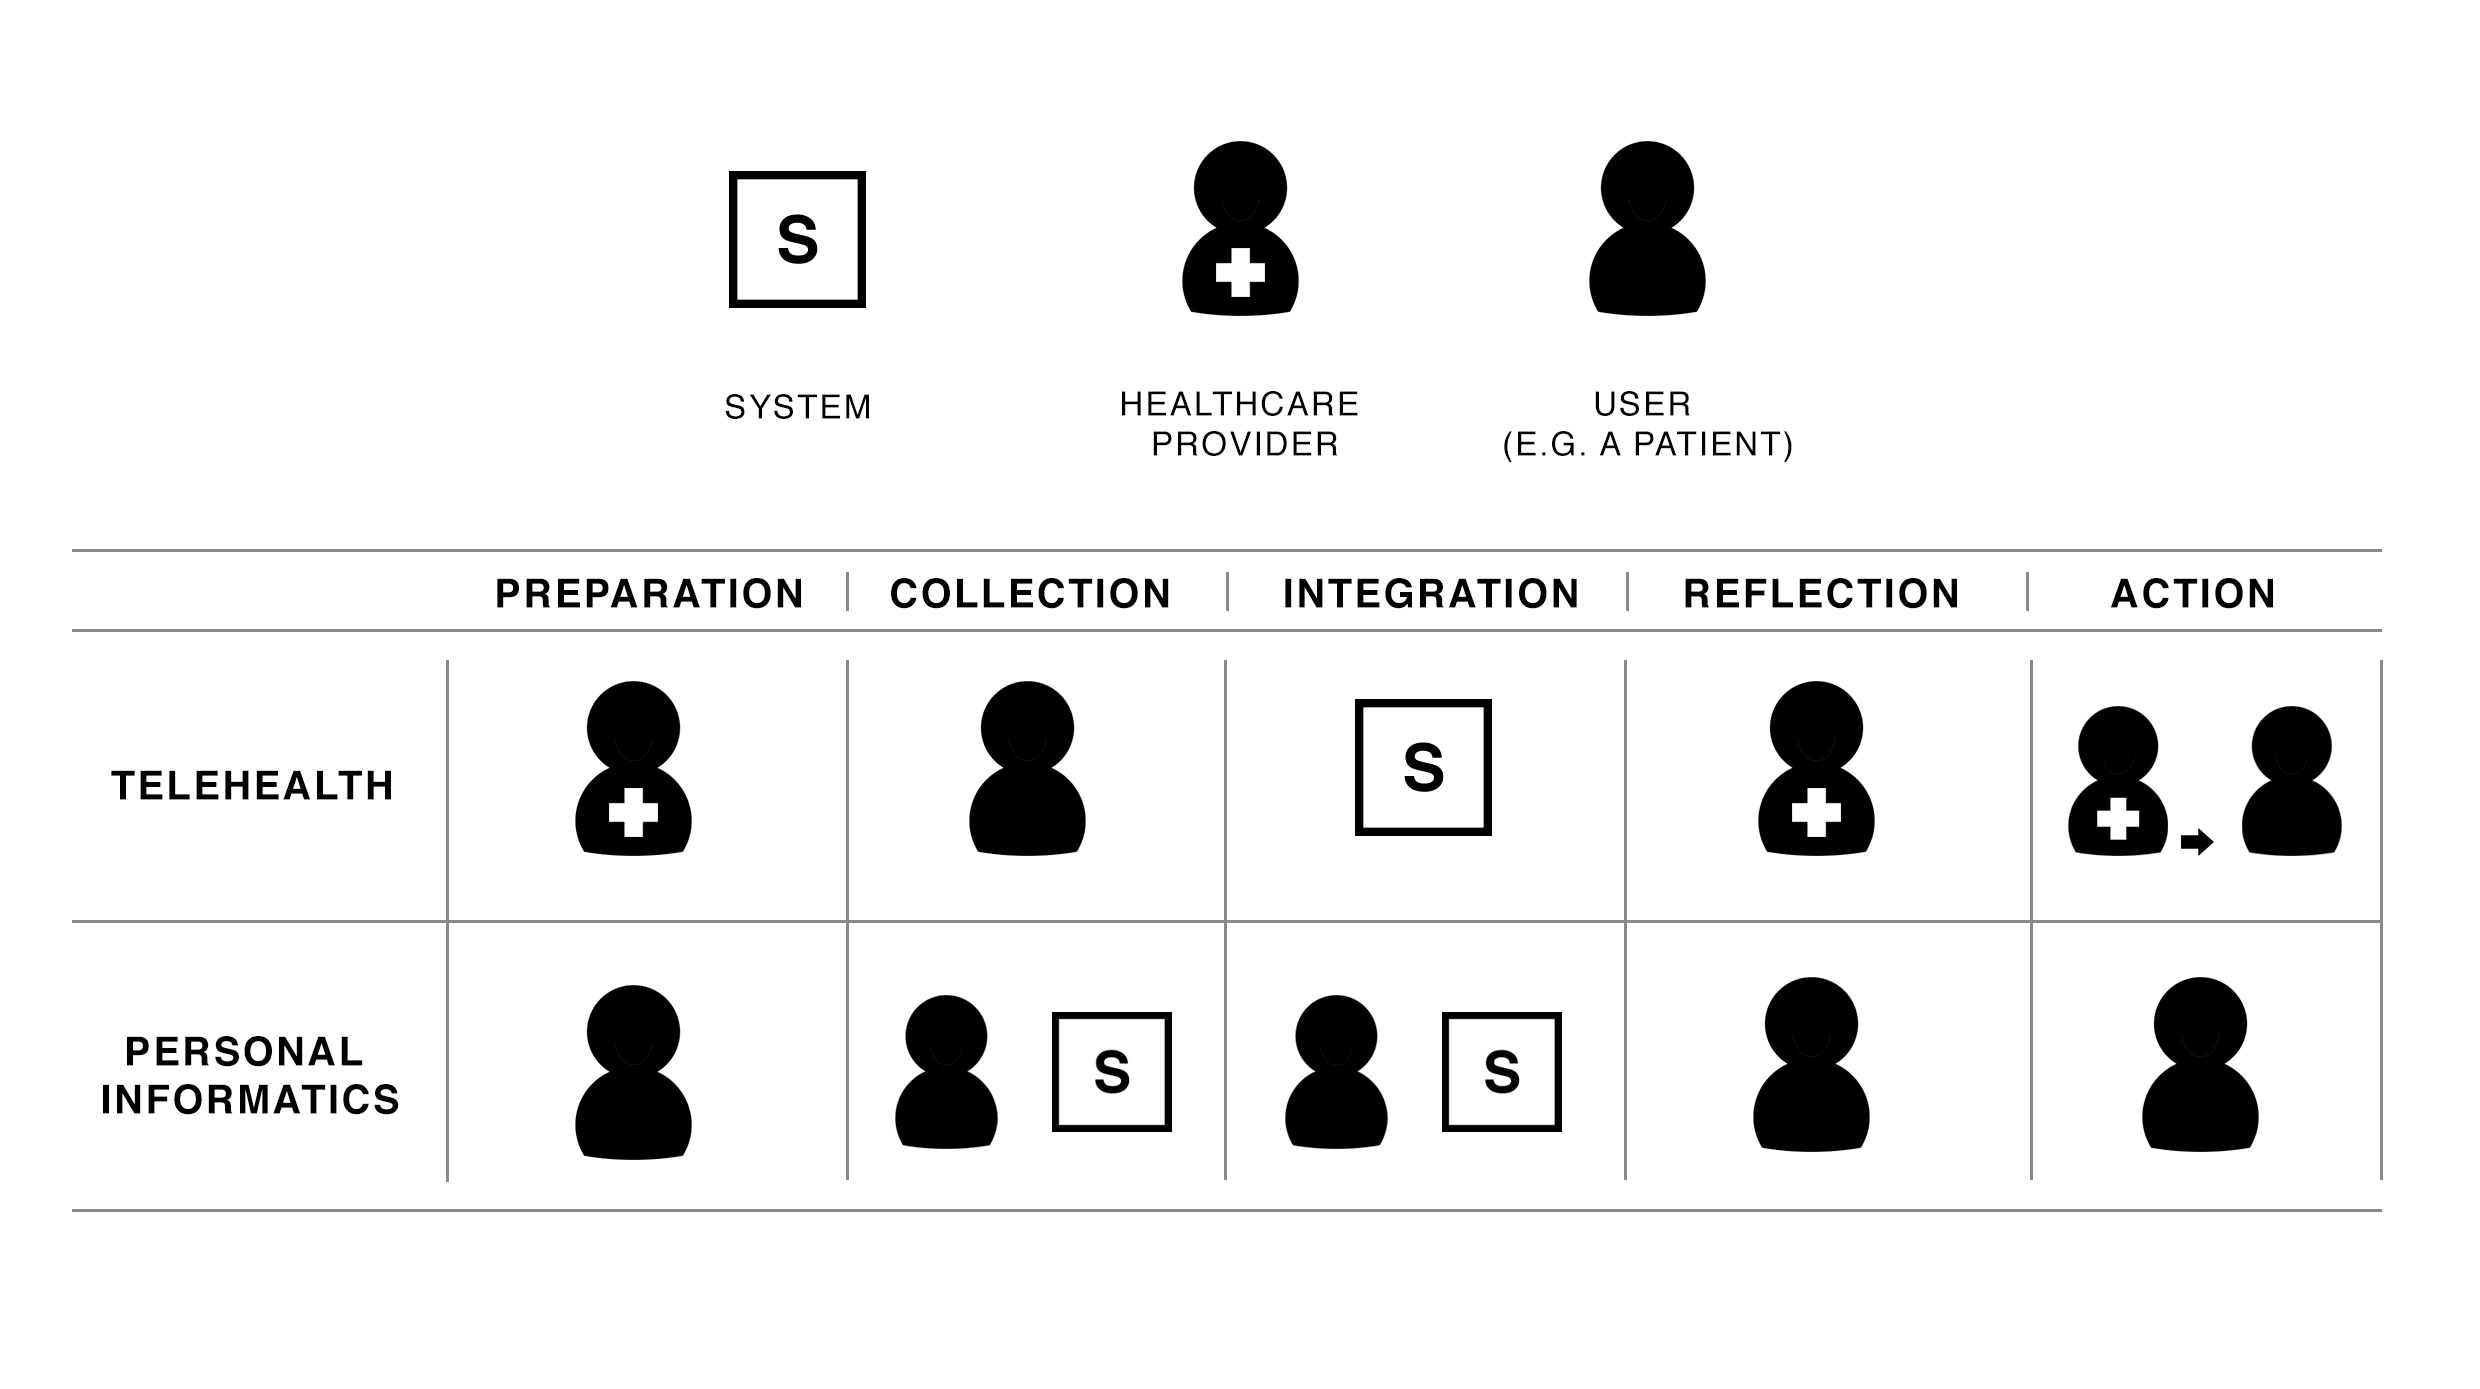
\includegraphics[width=0.9\columnwidth]{img/StakeholdersModel}
\caption{Stakeholders model bla bla}
\label{fig:StakeholdersModel}
\end{figure}

In telehealth, healthcare providers mandate and predefine what symptoms, how often and with what tool patients should track (\textit{preparation}). Patients collect both objective numerical (e.g. oxygen saturation measures) and subjective binary data (e.g. yes/no answers to whether dyspnea has increased more than usual) (\textit{collection}). The system integrates the data and based on predefined individual “normal ranges” flags data for follow-ups (\textit{integration}). Trained nurses or physicians review the self-tracked data (\textit{reflection}) in telehealth and if needed contact and advise the patient on potential initiation of treatment (\textit{action}) \cite{piloting, pedone}. 

Epstein et al. found that \textit{collection}, \textit{integration} and \textit{reflection} are ongoing processes that can occur simultaneously and categorize these activities as \textit{tracking and acting}. They further divide the \textit{preparation} stage into \textit{deciding} (deciding to self-track personally relevant data) and \textit{selecting} (selecting a tool to track with) and integrate \textit{lapsing} (e.g. due to an oversight or holidays) and \textit{resuming} into their \textit{Lived Informatics Model} \cite{Epstein2015, Rooksby2014}. 

While Li et al.’s and Epstein et al.’s work describes the different stages self-trackers transition between, Rivera-Pelayo et al. discuss Personal Informatics in light of reflective learning theory (or learning by reflection) \cite{Rivera}. Based on the work of Boud et al., they propose a framework consisting of three dimensions in which technology can be integrated to support reflection: (1) \textit{Tracking}, (2) \textit{triggering} and (3) \textit{recalling and revisiting}. Rivera-Pelayo et al. describe \textit{tracking} as logging data that serves as the basis for the reflective process. The data can both be experiences (e.g. feelings or physiological data), but also outcomes (e.g. gained insight or changes in behaviour). \textit{Triggers} have the purpose of raising awareness and detect discrepancies. These are related to the initiation of reflection based on the logged data. Finally, enrichment and data presentation facilitates \textit{recalling and revisiting} past experiences. 

We use the \textit{Lived Informatics Model} \cite{Epstein2015} and Rivera-Pelayo’s framework as an analytical lens to identify user needs and barriers for self-tracking in the following. We further aim to provide an understanding of, how technology can be used to support people in their self-tracking efforts. 

\subsection{Preparation} 
The \textit{preparation} stage includes includes people getting motivated to track (e.g. because of goal they have in mind), which guides the decision on, what data to track and selecting the tool to track with. 

\subsubsection{Motivation and Goals} 
As described by Epstein et al., people self-track for various reasons, but not all people self-track with a concrete goal in mind \cite{Epstein2015}. One example is people, who track out of natural curiosity about what their data might reveal about themselves \cite{Li2010, Epstein2015}. We refer to this as self-tracking for \textit{life experience}. From the literature, we classified four main drivers for sustained tracking among people with a health-related condition: (1) \textit{documentation} (e.g. to create records for their healthcare providers \cite{Ancker2015}), (2) \textit{communication} (e.g. to communicate their condition to family members \cite{MacLeod2014}), (3) \textit{self-knowledge and advice} (e.g. to get a sense of the current state of their condition or to get advice from their healthcare-provder \cite{MacLeod2014, Ancker2015}) and (4) \textit{self-improvement} (e.g. to change or maintain a behaviour in order to improve well-being or lifestyle \cite{MacLeod2014, Ancker2015, Chung2016}).

Barriers to motivation include strong emotional adversity to reflection on data, because it reminds people of negative aspects of their illness \cite{Li2010, Ancker2015}, tracking the wrong data or not tracking well enough to gain benefits \cite{Chung2015}, effort \cite{Choe2014, Patel2012}, reliability and relevance \cite{Oh2015, piloting, Epstein2015} and mismatches between subjective feeling and objective measures \cite{Ancker2015}. 

\subsubsection{Selection of Data and Tool} 
Previous studies show that, sometimes healthcare providers give little support on what symptoms to track and how to track (e.g. frequency of tracking) \cite{Patel2012}. This is an issue in health conditions that involve many symptoms that arise unexpectedly, where patients have to decide on additional symptom tracking \cite{Patel2012, Chung2016}. Trackers use tools, such as notebooks, health diaries and specific applications to do additional tracking or sometimes develop tools themselves that are cumbersome and incomplete \cite{Patel2012}. This later affects the \textit{integration} and \textit{reflection} stages, where healthcare providers struggle with interpreting data sets with additional and not always relevant information \cite{Chung2015, Chung2016}.

Little is known about what motivates to self-track in telehealth. As previously mentioned (See Figure \ref{fig:StakeholdersModel}), the decision on what to data track and which tool to use, is in telehealth context decided by a healthcare provider. Rivera-Pelayo et al. mention that selection of what data to track has an effect on the acceptance from the user and the efficiency of learning by reflection \cite{Rivera}.

\subsection{Collection} 
The \textit{collection} stage deals with logging of the data. Logging too many things can be challenging and lead to tracking fatigue \cite{Choe2014, Patel2012}, but since logging data is the basis for triggering and supporting \textit{reflection}, it is of importance to choose as unobtrusive a method as possible, which is sufficiently reliable \cite{Muller}. We previously described self-tracking as logging data (either objective or subjective) during concrete episodes over time. We now distinguish between data being either automatically logged (e.g. physiological sensors that log heart rate) and manually logged (e.g. self-reporting feelings or ideas). 

\subsubsection{Manual Logging}
Manual logging requires responsibility and motivation that has to be kept over time from trackers and can therefore be burdensome compared to automatic logging \cite{Li2010, Muller}. Some self-trackers find manual logging time consuming and requiring effort \cite{Ancker2015}, hampering incorporation of tracking into daily routines \cite{Verdezoto2015, Ancker2015}. One example is, when objective data has to be manually logged, it can require preparation time, e.g., resting before taking physiological measures, which increases time and effort \cite{Verdezoto2015}. Data granularity impede logging, when trackers overthink, while trying to rate mood on a scale from 0 to 10 \cite{Oh2015} and lack of baseline to compare with cause difficulties for trackers with chronic conditions, when self-reporting on severity of symptoms, because they are constantly symptomatic \cite{piloting}. Another downside of manual logging is that sometimes self-trackers postpone manual logging \cite{MacLeod2014}, which induces recall bias that that affects the data reliability. 

\subsubsection{Automatic Logging}
Automatic logging shifts the effort from the trackers to the technology. It allows for configuration of frequency and precision, but also implies challenges in terms of filtering and aggregating the large amounts \cite{Muller}. One of the main downsides of automatic logging is that it might reduce awareness and self-reflection \cite{Choe2014, Li2011}.

\subsection{Integration}
The \textit{integration} stage can be more or less apparent to the tracker depending on whether integration is automatically done by the system, requiring less effort from the self-tracker \cite{Li2010}. Self-trackers sometimes postpone data exploration when integration does not happen automatically, since it involves tedious tasks, such as cleaning up data, formatting and running statistical tests \cite{Choe2014, Chung2015, Li2010}. 

Systems that require manual integration expect the user to be able to analyse the data and ascertain the best way of creating a representation. This is of interest to curiosity-driven self-trackers that want to integrate data manually and explore the novel insights that data can offer them. In contrast, self-trackers with a goal know what they are looking for in the data and strive at using automatic integration systems allowing them to concentrate on reflection. The manual integration process is an iterative process of moving back and forth between representation creation and reflection \cite{Whooley2014}. 

\subsection{Reflection}
In the \textit{reflection} stage, self-trackers reflect on the collected and integrated data by looking, exploring or interacting with visualizations of it \cite{Li2010}. While literature points at many different definitions of reflection, Fleck \& Fitzpatrick identified five different ‘levels of reflection’ (R0-R4) that indicate what types of activities and behaviours can be associated with reflection \cite{Fleck}. Levels consist of (R0) describing or stating without being reflective (\textit{description}), (R1) describing with explanations in a reportive or descriptive way (\textit{reflective description}), (R2) seeing things from different perspectives and trying to identify relationships (\textit{dialogic reflection}), (R3) changing original point of view due to gained knowledge (\textit{transformative reflection}) and (R4) seeing the wider perspective beyond the immediate context (\textit{critical reflection}). While higher level indicates being more reflective, lower levels are prerequisites for becoming more reflective. 

\subsubsection{Conditions for Reflection}

One of the condition for reflection is creating and allowing for time to reflect \cite{Fleck}. Li et al. distinguish between short-term reflection, where the self-tracker reflects immediately after logging the data and long-term reflection that might occur several days or weeks after \cite{Li2010}. While short-term reflection makes the tracker aware of the current status, long-term reflection allows for higher levels of reflection (at least R2), since the tracker can compare logged data between different times and explore trends and patterns. 

Several authors mention that the one reflecting should be open-minded and willing to reflect \cite{insertTwoStudiesHere}. As mentioned by xx, in some literature there is an implicit assumption that \textit{skills} (such as critical analysis and evaluation) are necessary to engage in reflection \cite{insertTwoStudiesHere, Rogers}. Fleck \& Fitzpatrick mention that reflection can be developed with time and with the right support \cite{Fleck}. 

The reflective process further needs a trigger. People often need a reason (e.g. a purpose) or at least an encouragement to reflect \cite{Fleck, Mols}. In psychology, Festinger’s cognitive dissonance theory describes, how a mismatch (psychological discomfort or dissonance) between an individual's attitude and behaviour can lead to rethinking one’s attitude and behaviour \cite{Rivera}. The dissonance triggers reflection can be actively triggered (system explicitly tries to catch the user’s attention by highlighting a certain mismatch) or passively triggered (system only presenting the data and relying on the user to detect something that starts a reflective process). Dissonance may occur due to comparison between current level and a recommended level or goal, but some might prefer such comparison in response to oneself. For example, some self-trackers prefer to interpret their data in light of their own personal and medical history and/or symptoms, rather than striving for provider-recommended “normal ranges” \cite{Ancker2015}. 

In the following we describe different ways to trigger and support reflection identified in our literature review. 


\subsubsection{Reflective Questions or Prompting}
One way of supporting reflection is through the use of reflective questions or prompts. Simply asking people to provide justification or explanation for e.g. events or actions supports at least \textit{reflective description} (R1) \cite{Fleck}. The presence of another person can encourage reflection, especially in a dialogue among two “uneven partners” (i.e. two people not sharing the same understanding or experience), where one takes the role of asking questions. 

Systems can also take this leading role of asking questions, but opposed to the previously mentioned example, where reflection among two people can be “dialogue driven”, the systems often only pose  an initial reflective question \cite{Mols}. An intelligent system could further support reflection through follow-up questions. Another ways to foster reflection is by prompting questions triggered by automatically logged context data \cite{Fleck}. Presenting data that is not usually visible encourages people to see things from another perspective and can potentially lead to looking for relationships and patterns (R2). 

\subsubsection{Visualizations}
Despite simply looking at data is not considered reflective according to Fleck \& Fitzpatricks’ levels of reflection, creating representation of data is considered a prerequisite to support higher reflective levels. Visualizations of data can help people in exploring their information and gaining insights \cite{Li2010, Choe2014}. 

When designing visualizations, it is important to consider under which conditions reflection is to take place (e.g. time and effort expected from the user, skills and purpose for reflection) \cite{Cuttone, Muller}. Li et al. identified six types of questions people ask about their self-tracked data \cite{Li2011}. These are, getting to know (1) status (what is current status?), (2) history (what has status been in the past?), (3) goals (what goal is appropriate to pursue?), (4) discrepancies (how does current status compare to goal?), (5) context (what affects current status?), (6) factors (how are different variables related?). Depending on the conditions, supporting both simple (e.g. status charts) and detailed visualizations (e.g. of time series) can be important \cite{Muller, Cutone}.

Often people want to obtain answers to their question (e.g. status) without spending too much time or effort, which can be done on a simplified dashboard representation that allows for a quick overview \cite{Cutone}. Müller et al. found that people use status charts to quickly get an overview of their data and use it as a starting point for exploration \cite{Muller}. Comparison charts were requested in the study to benchmark against other people in the sense-making process and to assess success. However, as previously mentioned, some prefer that such benchmarking occurs in response to oneself \cite{Ancker2015}. 

Visualization of time series data support revisiting and analyzing past experiences (history) and can trigger storytelling about experiences behind data \cite{Rivera, Muller}. It can foster reflection on global trends e.g. on upward and downward trends or deviations from a historical normal (suggesting a problem) \cite{Rivera}. Cuttone et al. mention that human behavior is often characterized by periodic patterns, but that time series graphs do not facilitate exploring such patterns \cite{Cuttone}. They instead propose using calendar heatmap representations using different color shades to indicate variable values. Visualizations of multiple time series can support reflection on how multiple variables are related or how multiple variables change over time \cite{Cuttone}. 

Visualizations of time series can further be combined with discrete events \cite{Sorensen} to support reflective description (R1). Barriers for reflection include that tools to not always support either simple visualizations of data or more complex features (e.g. filtering data to focus on a subset of data, zooming out to get an overview or comparing multiple variables) \cite{Li2011, MacLeod}. 

\subsubsection{External activities}
While reflection is an internal process, it can occur when trying to externalize thoughts and feelings e.g. in diaries or during reflective writing \cite{Mols}. These activities are often descriptive or emotional (R1). Recording reflection outcomes for later revisiting and reflection on gained insights has been proposed as another way to support reflection \cite{Isaac, Muller}. Isaac et al. found that allowing for writing down thoughts helped people explore and understand their feelings \cite{Isaac}. 

\subsection{Action} 
People decide what \textit{action} to take based on the findings from the \textit{reflection} stage. Trackers who have other motivations than behaviour change, e.g. self-understanding, do not reach this stage \cite{Epstein2015}. Trackers who track for self-improvement sometimes lack the knowledge necessary to identify the appropriate actions to take, such that they can regulate their progress towards their behaviour change goal. This happens either because they collect irrelevant data \cite{Choe2014, Chung2015} (e.g. food and symptoms, instead of ingredients that trigger the symptoms) or because they need actionable (expert) advice \cite{Verdezoto2015, Li2010, Oh2015}. Most Personal Informatics systems do not provide actionable advice \cite{Chung2015, Li2010, Verdezoto2015} and trackers then seek out this advice from healthcare providers \cite{Li2010}.

\section{Research area}

In summary, previous literature shows user needs and concerns during tracking activities, but little is known about these aspects when tracking is monitored by a healthcare provider. It is unclear how concrete design decisions regarding entry and interaction with data affect reflection in such case. In study 1 we investigate user needs and concerns during tracking activities in telehealth context. Based on these findings we redesign the system to support patients in reflecting during data entry and interaction. 
